\chapter{تحلیل نیازمندی و معماری}

هدف اصلی پروژه ما طراحی و پیاده سازي سامانه‌اي است که بتوان توسط آن شبکه‌های کامپیوتری را پایش کرد. سامانه ذکر شده باید علاوه بر داشتن ویژگی‌های یک سیستم پایش شبکه، باید استفاده آن برای کاربر راحت و با کمترین دانش فنی قابل استفاده باشد. براي این که بتوانیم چنین سامانه‌اي را طراحی کنیم ابتدا باید نیازمندي‌هاي سامانه را تشخیص دهیم و سپس معماري کلی سامانه موردنظر خود را بر اساس تکنولوژی‌های انتخابی به دست آوریم.
\\
در این فصل ابتدا نیازمندی‌ها ذکر می‌شوند. بعد از آن به بررسی و انتخاب تکنولوژی توسعه نرم افزار می‌پردازیم. و درنهایت معماری نرم افزار را ترسیم می‌کنیم.



\section{تحلیل نیازمندي}
%% 2 

 بر اساس مطالعاتی که انجام شده و مطالب فصل قبل این سامانه باید قابلیت‌های زیر را داشته باشد:

\begin{itemize}
    \item کشف شبکه و ترسیم بصری آن برای ادراک بهتر توسط مدیر شبکه
    \item توانایی تنظیم پارامترها از جمله حد آستانه‌های عناصر تحت مدیریت بر اساس رفتار غیرمتعارف توسط مدیر شبکه و دوره تناوب جمع آوری اطلاعات از عناصر
    \item جمع آوری اطلاعات مدیریتی و پردازش آن‌ها جهت تولید اطلاعات قابل فهم توسط مدیر شبکه
    \item ایجاد یک رابط بصری مطلوب تحت وب و نمایش اطلاعات قابل فهم 
    \item فراهم آوردن حداقلی امنیت سیستم با استفاده از (\lr{SNMPv3} و پروتکل‌های دیگری که ایمن هستند)
    \item مقیاس پذیری سیستم جهت کارآمد بودن در هنگام افزایش وسعت شبکه
    \item فراهم آوردن یک مکانیزم هشدار با استفاده از حد آستانه‌های تعریف شده
\end{itemize}

\newpage

به طور خلاصه هدف از انجام این پروژه توسعه یک ابزار پایش شبکه با ویژگی‌های پایه‌ای فوق است. به عبارتی هدف، افزودن یک امکان جدید به پروژه‌های موجود و پیاده سازی آن نیست، اما از زبان‌های برنامه نویسی و تکنولوژی‌های بروز در مقایسه با پروژه متن باز زبیکس استفاده خواهد شد. به عبارت دیگر این پروژه از ابتدا بدون استفاده از کدهای متن باز موجود توسعه داده خواهد شد.



\section{بررسی و انتخاب تکنولوژی}
%% 4





\newpage

\section{معماری سامانه}
%% 2




با توجه به مطالبی که در این فصل تا به اینجا گفته شد، سامانه پایش شبکه‌های کامپیوتری به ماژول‌های زیر تقسیم می‌کنیم \cref{fig.11}. ابتدا یک ماژول تحت عنوان هسته \lr{SNMP} در نظر گرفته می‌شود که وظیفه مدیریت پیام‌ها و پیاده‌سازی پروتکل به یک زبان برنامه نویسی خاص است.




\begin{figure}[!h]
\centering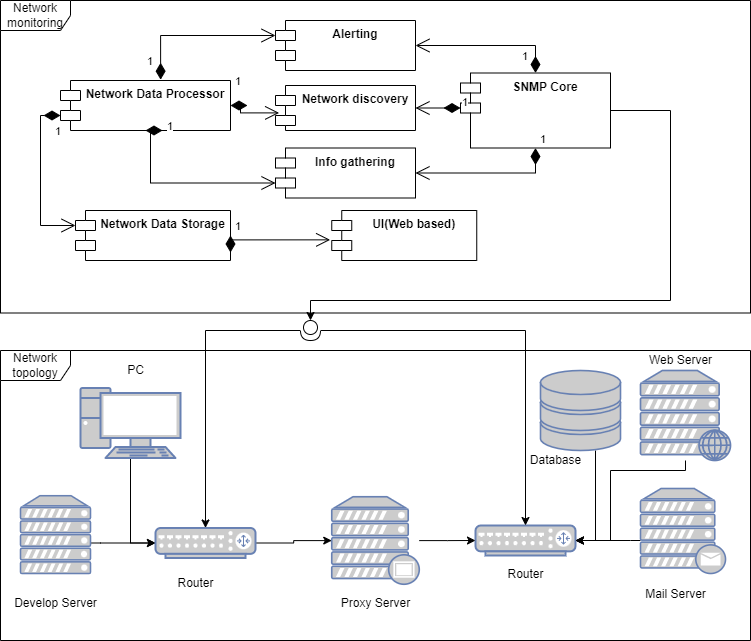
\includegraphics[scale=.55]{./diagram}
\caption{نمودار بلوکی اجزای سامانه}\label{fig.11}
\end{figure}


سپس ماژول کشف عناصر تحت مدیریت شبکه را در نظر گرفته می‌شود، که به کمک ماژول هسته وظیفه جمع آوری اطلاعات ساختاری شبکه را بر عهده دارد. بعد از آن ماژول جمع آوری اطلاعات دستگاه‌های مختلف، عملکرد کل شبکه را رصد می‌کند. حال اگر زمانی با توجه به وجود نوتیفیکیشن‌ها نیاز به هشدار وجود داشت، از ماژول هشدار استفاده می‌شود. 


نکته حائز اهمیت در رابطه با سه ماژول آخر این است که هر ماژول از ماژول هسته و همچنین ماژول ذخیره‌سازی اطلاعات شبکه تغذیه می‌شود. همچنین اطلاعاتی که هر ماژول بدست می‌آورد تحویل ماژول ذخیره‌سازی اطلاعات شبکه می‌دهد. در ماژول ذخیره سازی اطلاعات شبکه نیز اطلاعات در پایگاه‌های داده ذخیره می‌شوند، تا برای ماژول پردازشگر اطلاعات شبکه قابل بهره برداری باشد.

در پردازشگر اطلاعات شبکه نیز، اطلاعات خام دریافتی از ماژول ذخیره سازی اطلاعات شبکه پردازش می‌شوند تا اطلاعات قابل فهم توسط مدیر استخراج شود. حال باید اطلاعات تولید شده به ماژول رابط کاربری داده شود.

ماژول رابط کاربری نیز در قالب یک وب سایت و فراهم آوردن یک پنل ورودی مدیر شبکه نیز اطلاعات ساختاری شبکه، پایش شبکه و هشدارها را نمایش می‌دهد. همچنین از طریق آن می‌توان پارامترهای مختلف برای عناصر مختلف تنظیم و اقدام به اسکن کل شبکه کرد.

اما نیاز است که یک رابطی بین شبکه و سامانه مذکور باشد. در شکلی که بررسی شد، سامانه به یک شبکه فرضی از طریق روترهای آن متصل است. در واقع جمع آوری اطلاعات از شبکه و دریافت نوتیفیکیشن‌ها از طریق ماژول هسته \lr{SNMP} امکان پذیر خواهد بود.






\section{خلاصه}
% 1


خلاصه در اینجا قرار می‌گیرد.

